\subsubsection{Spectrogram ROIs}
Spectrum ROIs apply a curve fitting whereas Spectrogram ROIs do not. When applying a ROI to a spectrogram it sums the counts from all the channels within its bounds and do so for every row in the spectrogram. The results are displayed in count rate, as the number of counts are normalised to the save interval. This makes it easier to compare spectrograms recorded with different save intervals.

\begin{figure}[H]
    \centering
    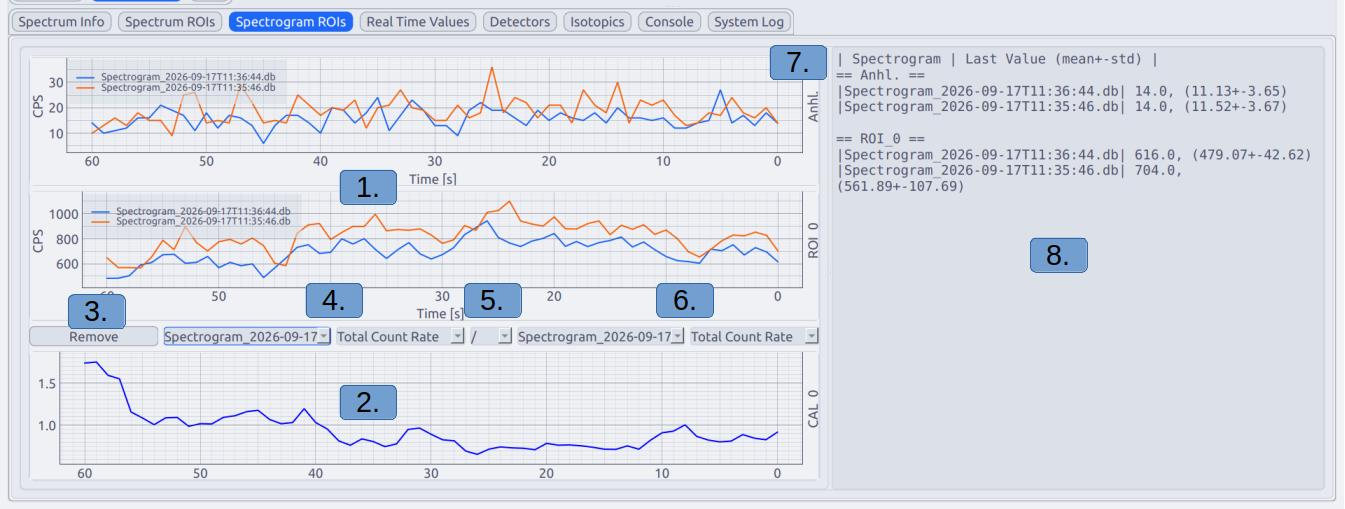
\includegraphics[width = .9\linewidth]{images/interface/spectrogram_rois.jpg}
    \caption{Spectrogram ROI tab showing two loaded spectrograms with two loaded ROIs. A \textit{Calculation ROI} is also added.}
    \label{fig:spectrogram_rois}
    \begin{flushleft}
        \begin{enumerate}
            \item Plots of two spectrogram ROIs evaluated on two separate spectrograms.
            \item Calculation ROI
            \item Button for removing the calculation ROI
            \item Settings for the first spectrogram in the calculation ROI. The first combobox lists loaded spectrograms and the second selects the data, total count rate or count rate from a ROI.
            \item Mathematical operations for comparing the ROI values are: \texttt{+}, \texttt{-} or \texttt{/}.
            \item Settings for the second spectrogram in the calculation ROI. These setting are the same as for the first (4.).
            \item ROI names. Calculation ROIs currently only have a tag containing a serial number on the form \texttt{CAL\_X}. Currently, they can not be renamed.
            \item ROI data in text form. Shown is the latest value and (mean+-std) calculated from the data shown in the plot.
        \end{enumerate}
    \end{flushleft}

\end{figure}

During mobile measurements LuRaCs offers the selection to monitor several ROIs simultaneously. For this e a 'Compact View' can be used. This is enabled under \texttt{View -> Spectrogram ROis -> Compact View}. This function strips all GUI elements from the plots, except the y-ticks and the plot itself.

\begin{figure}[H]
    \centering
    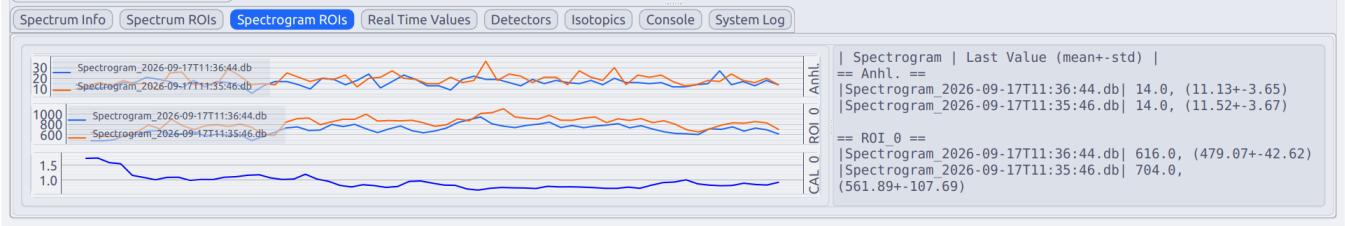
\includegraphics[width = .9\linewidth]{images/interface/spectrogram_rois_compact.jpg}
    \caption{Same spectrograms and ROIs as in \autoref{fig:spectrogram_rois} but in compact view.}
    \label{fig:spectrogram_rois_compact}
    
\end{figure}

\textit{Calculation ROIs} are plots calculated from the results of other ROIs. \textbf{These perform element wise operations and do not account for differences in measurement parameters}. Element 0 from ROI 0 is combined with Element 0 of ROI 1, regardless of measurement date or spectrogram save interval.